\chapter{مرور ادبیات مسئله}
\section{دسته‌بندی روش‌های موجود برای مسئله}
در طی چهار دهه گذشته روش‌های گوناگونی برای مسئله \gls{atm} پیشنهاد داده شده است.
با وجود این که هدف نهایی هر سیستم \gls{ATM} استخراج حالت نوشتاری موسیقی از روی
سیگنال‌های صوتی هست ولی اکثر راه‌حل‌های موجود تلاش می‌کند با رسید به یک هدف
میانی مسئله را حل کنند. با توجه به ماهیت این هدف‌های میانی و ساختار آن‌ها
می‌توان این روش‌ها را به چهار دسته کلی تقسیم کرد:
\begin{itemize}
    \item در سطح فرم
    \item در سطح نت
    \item در سطح جریان
    \item در سطح نماد
\end{itemize}

آوانویسی در سطح فرم یا \gls{mpe}، تخمین تعداد و \gls{pitch} نت‌های موجود در هر
یک فرم زمانی است. این فرم‌ها معمولا طولی در حدود چند میلی ثانیه دارند. هرچند این
تخمین معمولا برای هر فرم به صورت جدا انجام می‌شود ولی اطلاعات زمینه‌ای معمولا در
یک مرحله‌ پس‌پردازیش برای روی نتیجه به دست آمده اعمال می‌شوند تا دقت را افزایش
دهند. روش‌هایی که در سطح فرم تلاش می‌کنند که آوانسی را انجام دهند از مفهوم نت
استفاده‌ای نمی‌کنند و معمولا با هیچ فهموم موسیقیایی درگیر نمی‌شود.

حجم زیادی از روش‌های موجود در سطح فرم کار می‌کنند. روش‌هایی مانند پردازش سیگنال
به صورت سنتی \cite{emiya2009multipitch,su2015combining}، مدل‌های برپایه احتمال
\cite{duan2010multiple}، روش‌های برپایه بیز \cite{peeling2009generative}، \gls{nmf}
\cite{smaragdis2003non,vincent2009adaptive,benetos2013automatic,fuentes2013harmonic}
و روش‌های برپایه \gls{nn} \cite{sigtia2016end,kelz2016potential}. تمام این
روش‌ها نقاط قوت و ضعف خود را دارند و هنوز روشی به عنوان روش واحد انتخاب نشده
است. برای مثال روش‌های بر پایه پردازش سیگنال ساده‌تر و سریع‌تر هستند و قابلیت
تعمیم بالاتری به سازهای مختلف دارند. در حالی که روش‌های بر پایه \gls{dl} بر روی
یک ساز خاص، مثلا پیانو، به نتایج بهتری دست یافته‌اند. روش‌های بیضی می‌توانند
مدل‌سازی کاملی از فرآیند تولید صوت ارائه دهند، در حالی که به شدت پیچیده‌تر و
کندتر هستند.

آوانویسی در سطح نت، یک مرحله از \gls{MPE} سطح بالاتر هست از این جهت که این
روش‌ها فقط وجود یا عدم وجود نت در یک فرم را بررسی نمی‌کنند، بلکه فرم‌ها را به هم
وصل کرده و نت‌ها را در طول زمان بررسی می‌کنند. در \gls{ATM} معمولا هر نت را با
سه ویژگی \gls{pitch}، onset و offset مشخص می‌کنند \cite{klapuri2007signal}. با
توجه مبهم بودن offset در نت، در بعضی از سیستم‌ها، معمولا در نظر گرفته نمی‌شود.
در نتیجه مدل فقط \gls{pitch} و onset را پیش‌بینی می‌کنند.

حجم زیادی از روش‌های در سطح نت معمولا پس‌پردازیش‌هایی بر روی خروجی یک سیستم
\gls{MPE} هستند. به عنوان روش‌های استفاده شده می‌توان از \gls{hmm}
\cite{nam2011classification} و \gls{nn} \cite{boulanger2012modeling} نام برد. در
پس‌پردازیش‌های انجام شده معمولا هر نمونه به صورت جدا بررسی می‌شود و رابطه بین
نت‌ها همزمان در نظر گرفته نمی‌شود که باعث تشخیص اضافه یا کمتر نت‌هایی می‌شود که
هارمونیک مشترک با نت‌های درست دارند. از این جهت روش‌هایی بر پایه مدل موسیقی
پیشنهاد شده است تا در ارتباط بین نت‌ها نیز در نظر گرفته شود
\cite{boulanger2012modeling, sigtia2016end}. بخش دیگری از روش‌ها نت‌ها را مستقیم
از روی سیگنال صوت استخراج می‌کنند. برخی دیگر ابتدا onset هر نت را پیدا می‌کنند و
سپس \gls{pitch} را بین آن‌ها تشخیص می‌دهند \cite{marolt2004connectionist}. برخی
دیگر حتی کل اطلاعات را با هم استخراج می‌کنند
\cite{cogliati2016context,ewert2016piano,hawthorne2017onsets}.

آوانویسی در سطح جریان یا \gls{mps} هدفش گروه بندی نت‌ها تخمین زده شده در
مجموعه‌ای جریان هست که هر جریان معمولا متناظر با یک ساز هست. این گروه از روش‌ها
ارتباط نزدیکی با \gls{iss} دارد. یکی از مزایای \gls{MPS} نسب به روش‌های قبلی
بررسی و تاثیر دادن \gls{timber} است. کارهای انجام شده در این سطح بسیار محدود
هستند.

تمام سه خانواده از روش‌های‌ توضیح داده شده خروجی اصطلاحا پارامتری دارند. علت این
نامگذاری این هست که این آوانویسی انجام شده، یکی از پارامترهایش سیگنال صوتی ورودی
هست. این آوانویسی‌ها با وجود این که تا حدی از مفاهیم مسیقیایی استفاده می‌کنند
ولی خروجی آن‌ها هنوز اختلاف زیادی با سطح مجردسازی انجام شده در \gls{sheet music}
دارد. مهمترین این اختلاف‌ها زمان هست که در هر سه روش در واحد ثانیه اندازه گرفته
می‌شود. در حالی که در موسیقی زمان در واحد ضرب اندازه گرفته می‌شود. همچنین
\gls{pitch} در فراکنس هست در حالی که در موسیقی معمولا هر نت نامی مانند دو بمل
دارد و باتوجه به گام قطعه تعریف می‌شود. در نهایت مفاهیمی مانند میزان، ضرب آهنگ،
تمپو، گام و هارمونی کاملا حذف شده‌اند.

هدف آوانویسی در سطح نماد این هست که خروجی سیستم، نمادگذاری قابل لمس برای انسان
باشد که تمام اطلاعات موسیقیایی لازم را در بردارد. خروجی مانند \gls{sheet music}.
آوانویسی در این سطح نیاز به درک عمیق مفاهیم موسیقی مانند هارمونیک و ریتم دارد.
ساختارهای هارمونیک مانند گام و آکوردها باعث تغییر شکل نمایش \gls{pitch} می‌شوند.
ساختارهای ریتمیک مثل ضرب و میزان باعث می‌شود که طول نت‌ها از ثانیه مستقل شود.

چندین مطالعه تلاش کرده‌اند که ساختارهای موسیقیایی را از روی سیگنال صوتی یا
\gls{MIDI} به دست آورند. با این وجود مطالعات خیلی کمی برای روی یک سیستم
آوانویسی کامل انجام شده است که از این مفاهیم استفاده کند.

با این وجود که روش‌های بسیار متفاوتی برای \gls{atm} وجود دارد ولی در دهه گذشته
بهترین دقت به دست آمده از دو خانواده از روش‌ها بوده است:
\begin{itemize}
    \item \gls{nmf}
    \item \gls{nn}
\end{itemize}
هر دو خانواده این مسائل برای مسائل بسیار متفاوتی مانند پردازش گفتار، پردازش
تصویر و سیستم‌های پیشنهاددهنده استفاده شده‌اند و نتایج بسیار رضایت بخشی به دست
آورده‌اند. در ادامه استفاده هر دو روش برای سیستم‌های \gls{ATM} بررسی می‌شود.

\section{روش‌های برپایه‌ی تجزیه نامنفی ماتریس}
ایده اصلی در روش‌ها بر پایه \gls{nmf} این است که یک نمایش دو بعدی نامنفی
زمان-فرکانس، مانند $V \in R_{\leq 0}^{m \times n}$، به شکل حاصل ضرب دو ماتریس
غیرمنفی، مانند $D \in R_{\leq 0}^{m \times k}$ و $A \in R_{\leq 0}^{k \times
n}$، نمایش دهیم. پس از این تجزیه می‌توان هر ستون ماتریس اول، $D$، را به یک نت نسب
دهیم و همچنین هر ستون ماتریس دوم، $A$، معلوم می‌کند که کدام نت‌ها در یک زمان خاص
فعال بوده‌اند. به بیان دیگر هدف پیدا کردن دو ماتریس نامنفی، $D$ و $A$، است به
گونه‌ای که فاصله $V$ و $DA$ حداقل شود. برای پیدا کردن این دو ماتریس معمولا با دو
مقدار تصادفی شروع می‌کنیم و در دنباله‌ای از به روزرسانی‌ها سعی می‌کنیم که این دو
ماتریس را پیدا کنیم. مثلا اگر از تابع خطای \lr{Kullback-Leibler} استفاده کنیم،
می‌توان نشان داد که قوانین به روزرسانی زیر برای $D$ و $A$ تضمین می‌کند که خطا
افزایش نیابد و مقدار هر دو ماتریس نامنفی بماند.
\begin{equation}
    A \leftarrow A \odot \frac{D^T(\frac{V}{DA})}{D^T J}
\end{equation}
\begin{equation}
    D \leftarrow D \odot \frac{(\frac{V}{DA})A^T}{J A^T}
\end{equation}

در روابط بالا $\odot$ نشان دهنده ضرب درایه به درایه است. همچنین کسر خطی نشان
دهنده تقسیم درایه به درایه است. $J \in R^{m \times n}$ نیز ماتریسی است که تمام
درایه‌های آن یک هستند.

پس از تجزیه می‌توان هر ستون نمایش زمان-فرکانس ورودی، $V$، به شکل ترکیب خطی‌ای از
ستون‌های $D$ بیان کرد. هر ستون $D$ نمایی از فرکانس‌های تولید شده توسط هر نت هست.
همچنین ستون‌های ماتریس $A$ ضرایب این ترکیب را بیان می‌کنند. فرض اصلی که تمام این
روش‌ها می‌کنند این است که اجرای نت‌ها برروی هم تاثیر کاهشی‌ای ندارند و خروجی
سیستم صرفا ترکیب صداهای تولید شده توسط هر نت است. در شکل زیر می‌توان نمونه‌ای
ماتریس‌های $D$ و $A$ به دست آمده از ورودی را مشاهده کنید. همچنین در نمایش مربوط
به ماتریس $D$ به خوبی می‌توان فرکانس پایه هر نت و همچنین هامونیک‌های مرتبط با آن
را مشاهده کرد. همچنین شباهت میان ماتریس $A$ و نمایش \gls{pianoroll} کاملا واضح
هست.
\begin{figure}
    \centering
    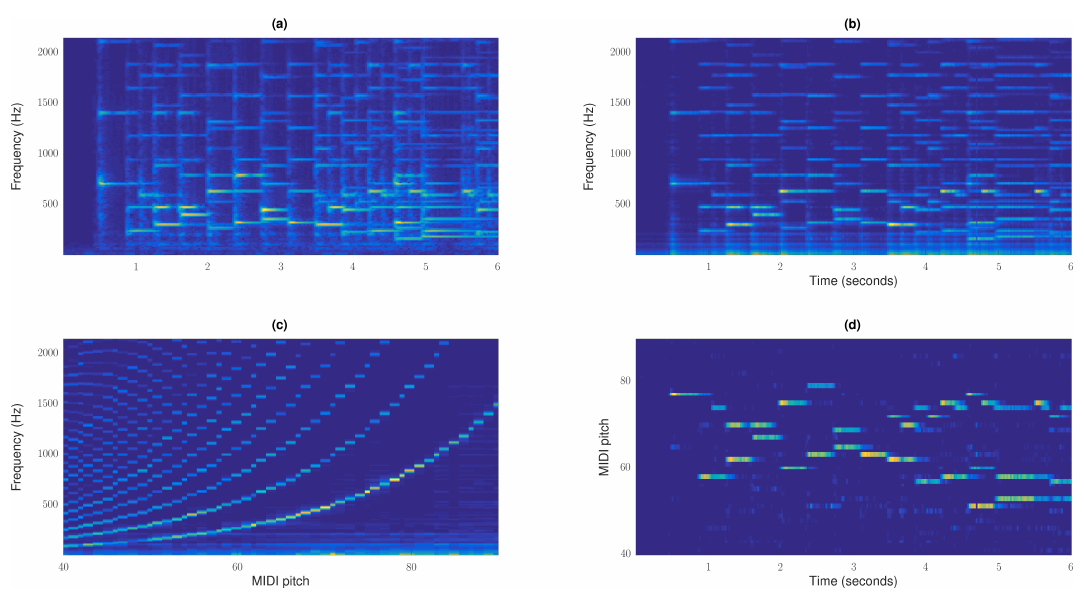
\includegraphics[height=8cm]{./statics/nmf_visualized.png}
    \caption{نمونه از انجام \gls{nmf} بر روی یک اسپتگرام ورودی.
a نمایش اسپکتوگرام ورودی است.
b اسپکتوگرام باز تولید شده است.
c و d به ترتیب ماتریس‌های D و A هستند.}
\end{figure}

برای حل مشکلات مسئله \gls{atm}، روش‌های مبتنی بر \gls{nmf} معمولا محدویت‌هایی در
عملیات تجزیه اعمال می‌کنند. برای مثال تلاش می‌شود که ماتریس $A$ تا حد ممکن یک
ماتریس تنک شود. این تنک سازی باعث می‌شود که نت‌هایی همزمان تشخیص داده شده محدود
شود و در نتیجه فقط نت‌هایی بهترین توصیف ممکن را می‌توانند ارائه دهند فعال فرض
می‌شوند. یک محدودیت دیگر این است که ممکن است ماتریس $D$ را سیستم مستقیم فرا
نگیرد. بلکه از یک ماتریس ثابت که دستی هر ستون آن متناظر با فرکانس‌های تولید شده
هر نت قرار داده شده است استفاده می‌شود.

\section{روش‌های برپایه‌ی شبکه‌ عصبی}
همانند دیگر مسائل مرتبط با حوزه تشخیص الگو، شبکه‌های عصبی تاثیر قابل توجهی بر
روی مسئله \gls{atm} و به صورت کلی‌تر حوزه \gls{mir} داشته‌اند. \glspl{nn}
توانایی یادگیری توابع غیرخطی پیچیده‌ را دارند که به آن‌ها برای حل مسائل کمک
می‌کند. با این وجود در مقایسه با حوزه‌ای مانند بینایی ماشین، سرعت رشد استفاده از
\gls{nn} برای حل مسئله \gls{atm} پایین بوده است. در ادامه تلاش می‌کنیم چند علت
این کندی را بررسی کنیم.

یکی از اولین استفاده‌ها از \gls{nn} برای حل مسئله توسط
\cite{marolt2004connectionist} ارائه شده است. بخش اصلی این مدل استفاده از شبکه
تاخیر زمانی بوده است که همانند یک \gls{cnn} در بعد زمان عمل می‌کند. هر چند
انتشار این روش به ۲۰۰۱ برمی‌گردد ولی در زمان انتشار، روشی موثر محسوب می‌شد و تا
سال‌ها سایر روش‌ها خود را با آن مقایسه می‌کرده‌اند.

این مدل ابتدا سیگنال‌های صوتی ورودی را توسط یک مدل شنوایی، که بسیار شبیه سیستم
شنوایی انسان کار می‌کند، تبدیل به یک نمایش زمان-فرکانس می‌کند. شیوه تبدیل به این
صورت است که ابتدا از یک بانک فیلتر استفاده می‌شود تا سیگنال صوتی به کانال‌های
فرکانسی مختلف تقسیم شود. مقدار این فیلترها به گونه‌ای انتخاب شده است که خروجی
بسیار نزدیک به گوش میانی انسان تولید کند. سپس خروجی هر فیلتر تبدیل به یک نمایش
احتمالی می‌شود. این تبدیل توسط مدلی انجام می‌شود که بسیار شبیه نرون‌های شنوایی
عمل می‌کند و بسیار از رفتارهای این نرون‌ها را مدل می‌کند. سپس این نمایش به یک
نوسان‌ساز انطباقی داده می‌شود تا بخش‌های فعال مرتبط با هر نت استخراج شود.

پس از استخراج بخش‌های فعال از ۷۶ \gls{nn} مجزا استفاده می‌شود تا تشخیص داده شود
کدام نت در هر مرحله فعال است. دلیل استفاده از ۷۶ خروجی این است که نت‌ها اکتاو
پایین پیانو کنار گذاشته شده است. دلیل حذف این نت‌ها دقت پایین تشخیص  این نت‌ها
است. همچنین استفاده از این اکتاو در اکثر قطعات موسیقی رایج نیست. برای همین
می‌توان فرض کرد که حذف آن‌ها در دقت کل سیستم تاثیر قابل توجهی نخواهد داشت. برای
این شبکه‌ها از ساختار تاخیر زمانی استفاده شده است که در بررسی‌های انجام شده
نتایج رضایت بخش‌تری نسبت به ساختارهای جایگزین نشان داده است.

همچنین از خروجی مدل شنوایی استفاده می‌شود تا شروع نت‌ها نیز تشخیص داده شود. برای
این کار از نرون‌های ضربه استفاده می‌شود. به این صورت که کدام از باندهای فرکانسی
پس از مقداری پس‌پردازش به یک نرون داده می‌شود. اگر ورودی نرون بیش از مقدار
آستانه تحریک شود، نرون یک ضربه در خروجی تولید می‌کند. سپس این ضربه‌ها توسط یک
شبکه \gls{mlp} بررسی می‌شوند تا ضربه‌هایی که حاصل شروع نت هستند شناسایی شوند.

همچنین در این سیستم نیاز به روشی برای تشخیص نت‌های تکراری حس می‌شود. برای همین
شروع نت‌های تشخیص داده شده و همچنین نت‌های تشخیص داده شده در هر مرحله به یک شبکه
\gls{mlp} دیگر داده می‌شود تا نت‌های تکراری را تشخیص دهد.

در نهایت از سیستم با استفاده از اطلاعاتی که استخراج کرده است تلاش می‌کند کشش و
همچنین شدت نت‌ها را پیش‌بینی کند. کشش نت‌ها از خروجی تشخیص نت‌ها به دست می‌آید.
وقتی مقدار هر خروجی متناظر با نت‌ها به زیر مقدار آستانه برسد، سیستم نت را تمام
شده فرض می‌کند. برای تشخیص شدت نیز از شدت هارمونیک اول هر نت استفاده می‌شود. در
ادامه شکلی که در ادامه آمده ساختار کلی این مدل ترسیم شده است.
\begin{figure}[ht]
    \centering
    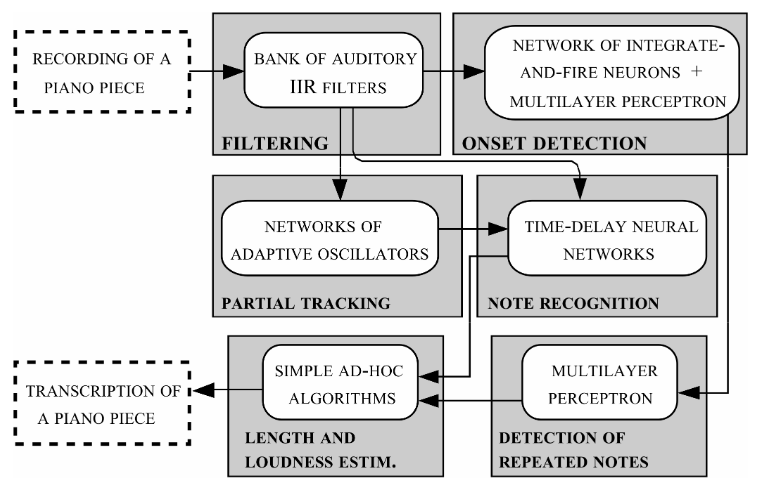
\includegraphics[height=8cm]{./statics/marolt2004connectionist_architecture.png}
    \caption{ساختار مدل استفاده شده در \cite{marolt2004connectionist}}
\end{figure}

ایده جالب دیگری که در \cite{bock2012polyphonic} داده شد این بود که از دو
\gls{spec} مختلف با دقت‌های مختلف در بعد زمان استفاده شود. برای محاسبه
\gls{spec} اول، دقت بالاتری در بعد زمان دارد، از پنچره‌ای به طول ۴۶/۴ میلی‌ثانیه
استفاده شده است. شبکه می‌تواند از این داده‌های با کیفیت‌تر استفاده کند تا شروع
نت‌ها و فعال بودن آن‌ها بهتر تشخصی دهد. \gls{spec} دوم از پنجره‌ای به طول ۱۸۵/۸
میلی‌ثانیه دارد. این \gls{spec} با وجود داشتن دقت پایین‌تر، می‌تواند توسط شبکه
استفاده شود تا رابطه‌های طولانی‌تر را فراگیرد. مثلا می‌توان شبکه بیاموزد که پس
از دو نت اول یک آکورد، دو و سل، وجود نت سوم آکورد، فا، محتمل هست.

همچنین برای محاسبه \glspl{spec}، ابتدا تابع \gls{STFT} بر روی سیگنال ورودی اعمال
می‌شود. سپس فرکانس‌ها در یک مقیاس لگاریتمی متناسب با هر نیم‌پرده، دسته بنده
می‌شوند. استفاده از نیم‌پرده بجای حالت‌های رایج‌تر مانند ربع‌پرده دو مزیت دارد.
اول این که اندازه هر ورودی تقریبا نصف می‌شود که خود باعث بار محاسباتی به شدت
کمتر و آموزش سریع‌تر شبکه می‌شود. همچنین باعث می‌شود که ورودی در مقابل تفاوت‌های
جزئی کوک بین پیانو‌های مختلف مقاوم شود و نیاز به کوک شدن تمام سازها با هم را حذف
کند.

\gls{spec} محاسبه شده سپس به یک شبکه سه لایه با ساختار \gls{blstm} داده می‌شوند.
توانایی این شبکه که در هر مرحله می‌تواند از همه اطلاعات گذشته و آینده استفاده
کند در این مسئله اهمیت بسیار بالایی دارد. برای مثال، برای تشخیص شروع نت‌ها فقط
اطلاعات مربوط به مرحله حمله کافی نیست و داشتن اطلاعات ادامه تغییرات سیگنال صوتی
نیز می‌تواند بسیار مفید باشد.

یک تفاوت جالب این مدل با سایر مدل‌ها این است که این مدل بجای انجام
\gls{classification}، از \gls{regression} برای تعیین نت‌های فعال استفاده می‌کند.
به این صورت که اگر مقدار تخمین زده شده از حدی بالاتر بود، نت فعال فرض می‌شود.
ادعا شده است که این استفاده از \gls{regression} به تشخیص نت‌های فعال واقعی از
هارمونیک نت‌های فعال کمک می‌کند و دقت نهایی سیستم را افزایش می‌دهد. در نهایت
شبکه با استفاده از \gls{gd} ساده و تابع \gls{mse} آموزش داده می‌شود. در شکل
زیر ساختار کلی این مدل نشان داده شده است.
\begin{figure}[ht]
    \centering
    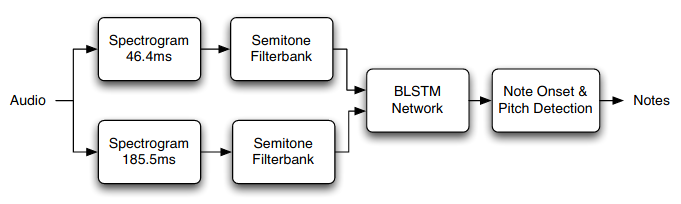
\includegraphics[width=12cm]{./statics/bock2012polyphonic_architecture.png}
    \caption{ساختار مدل استفاده شده در \cite{bock2012polyphonic}}
\end{figure}

در \cite{sigtia2016end} تلاش شد که این ارتباط بین نت‌ها با استفاده از یک مدل
موسیقیایی در کنار مدل صوتی مدل شود. از این روش در سیستم‌های \gls{asr} استفاده
می‌شود و تاثیر به سزایی دارد. برای ساخت مدل موسیقیایی اطلاعات نت‌های هر قطعه به
یک \gls{rnn} داده می‌شود تا بتواند پیش‌بینی کند در فرم بعدی چه نت‌هایی فعال خواهد
بود. ایراد این روش این است که مدل نیاز دارد که یک توزیع احتمالی بزرگ را یاد
بگیرد و استفاده کند. این توزیع، توزیع متناظر به فعال یا غیرفعال بودن هر کلاویه
پیانو هست که $2^{88}$ حالت دارد. برای مدلسازی این فضای احتمالی به این بزرگی، از
یک ساختار خیلی خاص استفاده شده است که این احتمال را به شکل دنباله‌ای از ضرب
احتمال‌های شرطی نشان می‌دهند. با این وجود، شبکه بهبود کمی نسبت به یک \gls{hmm}
نشان داد، که مجددا باعث شک در توانایی مدل‌سازی این ارتباطات می‌شود.

در \cite{kelz2016potential} توانایی شبکه‌های عصبی نسبتا ساده در حل مسئله
\gls{atm} بررسی شد. اولین موضوعی که بررسی شد، مقایسه تاثیر نمایش‌های مختلف
زمان-فرکانس به عنوان ورودی است. برای این مقایسه ابتدا سیگنال صوتی ورودی با
استفاده از چهار نمایش تبدیل مختلف تبدیل به نمایش‌ها زمان-فرکانس مختلف شد.
تبدیل‌های استفاده شده، تبدیل \gls{STFT} با دسته‌بندی‌های خطی، \gls{STFT} با دسته
بندی‌های لگاریتمی، \gls{STFT} با دسته‌بندی‌های لگاریتمی و مقیاس لگاریتمی و
\gls{CQT} هستند. سپس نمایش‌های به دست آمده به دو مدل با ساختارهای \gls{logistic
regression} و شبکه عصبی تک‌لایه داده شد تا آوانویسی را انجام دهند. دلیل استفاده
از مدل‌های با ساختار ساده کاهش توانایی استنتاج مدل و تمرکز بیشتر بر روی تاثیر
نمایش ذکر شده است. بر خلاف انتظار رایج، نمایش \gls{CQT} در مقایسه با سایر روش‌ها
دقت پایین‌تری ارائه کرد. در شکل زیر نتایج این مقایسه برای هر دو مدل نشان داده است.
\begin{figure}[ht]
    \centering
    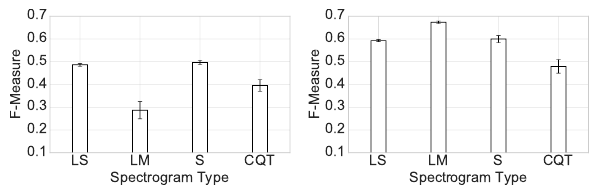
\includegraphics[width=12cm]{./statics/kelz2016potential_spec.png}
    \caption{بررسی تاثیر نحوه تولید \gls{spec} بر روی \gls{logistic regression} و \gls{nn}}
\end{figure}

همچنین تلاش شد تا جست‌وجوی نسبتا جامع بر روی \glspl{hyper parameter} مختلف بر
روی مدل‌های مختلف بر پایه \gls{nn} انجام شود تا تاثیر هرکدام را در مسئله
\gls{atm} بررسی کنند. نتایج نشان داد که مهم‌ترین \gls{hyper parameter} در مسئله
\gls{learning rate} است که با اختلاف از \glspl{hyper parameter} دیگر تاثیر بیشتر
در دقت خروجی مدل دارد. همچنین \gls{hyper parameter} با اهمیت دیگر \gls{spec}
ورودی شبکه است. در شکلی که در ادامه قرار دارد، تاثیر هر کدام از این مقدارها
مقایسه شده است.
\begin{figure}[ht]
    \centering
    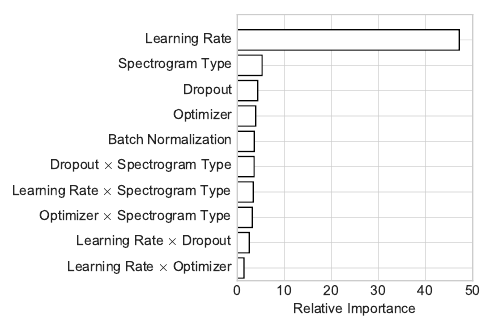
\includegraphics[width=12cm]{./statics/kelz2016potential_hp.png}
    \caption{نتایج تاثیر \glspl{hyper parameter} مختلف در دقت نهایی مدل}
\end{figure}

در نهایت از یافته‌های پیشین استفاده شد که مدلی تنها برپایه \gls{cnn} ارائه شود
که در زمان انتشار بهترین دقت منتشر شده را به دست آورده بود. ورودی این شبکه
\gls{spec} با دسته‌بندی‌های لگاریتمی و مقایس لگاریتمی هست. به ازای هر اکتاو ۴۸
دسته‌بندی استفاده شد. برای آموزش شبکه از تابع خطای \gls{cross entropy} و ADAM
استفاده شد.

در \cite{wang2017two} تلاش شد تا مدلی ارائه شود که از مزایی \gls{nn} و \gls{nmf}
با هم بهره ببرد. \gls{cnn} توانایی خود را در آوانویسی در سطح فرم به خوبی نشان
داده‌اند و دقتی بالاتر سایر روش‌ها به دست آورده‌اند. ولی برای آوانویسی در سطح
نت، \gls{nmf} همچنان از دقت بالاتری بهره‌مند هستند. برای همین تلاش شد در این مدل
از هر دو خانواده از روش‌ها به گونه‌ای استفاده شود که از نکات قوت هر دو بتوان
استفاده کرد. برای این منظور ابتدا از دو شبکه \gls{CNN} استفاده می‌شود تا
فرم‌هایی که نتی در آن‌ها شروع می‌شود را پیدا کنند و همچنین نت‌های فعال در آن
فرم‌ها مشخص شود. سپس با کمک یک مدل متبنی در \gls{NMF} این خروجی بررسی می‌شود و
نتیجه نهایی مدل تولید می‌شود.

ابتدا \gls{spec} مبتنی در \gls{CQT} تولید می‌شود. این نمایش زمان-فرکانس به دست
آمده به یک \gls{cnn} دو لایه داده می‌شود تا مشخص شود در هر فرم آیا نتی شروع
می‌شود یا خیر. در مرحله بعدی به ازای هر شروع نت تشخیص داده شده برشی از
\gls{spec} تولید شده به \gls{CNN} بعدی داده می‌شود که فرم حاوی شروع نت در وسط آن
قرار دارد. این شبکه ساختاری کاملا شبیه به \gls{cnn} مرحله قبل دارد تنها با این
تفاوت که بجای یک خروی ۸۸ خروجی دارد. این شبکه مسئول این است که تشخیص دهد که کدام
نت‌ها در این فرم وسط فعال شده‌اند. در شکل زیر ساختر \gls{CNN} نشان داده شده است.
\begin{figure}[ht]
    \centering
    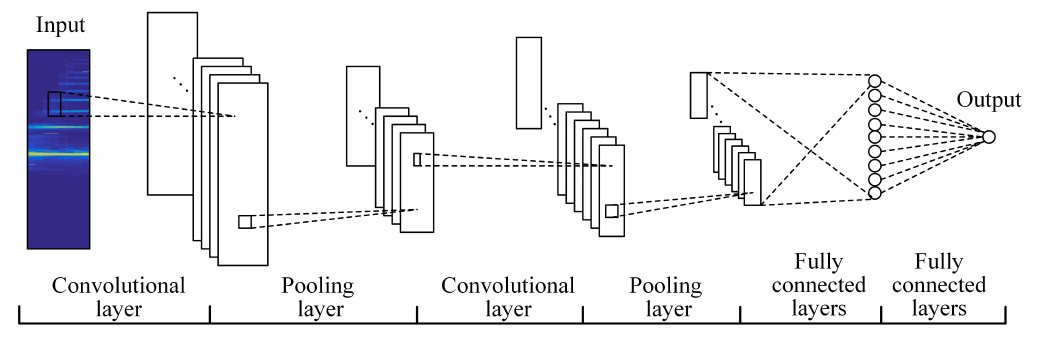
\includegraphics[width=12cm]{./statics/wang2017two_cnn.png}
    \caption{ساختار \gls{CNN} استفاده شده در \cite{wang2017two}}
\end{figure}

در قدم بعدی با استفاده از تجزیه \gls{spec} ورودی تلاش می‌شود تا دقت تشخیص‌های
انجام شده افزایش پیدا کند. $R_{t - T}^{t + T}$ برشی از \gls{spec} است که در آن
$t$ فرمی است که در آن شروع نت تشحیص داده شده است. $W_k$ قالب مرحله‌ی حمله اجرای
نت $k$ام تشخیص داده شده هست، از پیانویی که ضبط بر روی آن انجام شده است. این فرض
داشتن نمونه‌های اجرای جدای هر نت به ازای پیانوی استفاده شده که بزرگ‌ترین ضعف این
مدل محسوب می‌شود. $H_{t - T}^{t + T}$ نیز ماتریسی‌ است که فعالیت هر نت را نشان
می‌دهد. رابطه این سه ماتریس توسط رابطه زیر نشان داده شده است:
\begin{equation}
    R_{t - T}^{t + T} = \sum_{k} w_k H_{t - T}^{t + T}
\end{equation}

پس از محسابه $H$ درایه‌هایی که مقدار آن‌ها بیش از حد آستانه انتخاب شده باشد فعال
فرض می‌شوند. نکته قابل توجه دیگر این است که این مدل فقط شروع نت‌ها پیش‌بینی
می‌کند در مورد پایان نت‌ها تشخیص انجام نمی‌دهد. در شکل زیر ساختار کلی این سیستم
نشان داده شده است.
\begin{figure}[ht]
    \centering
    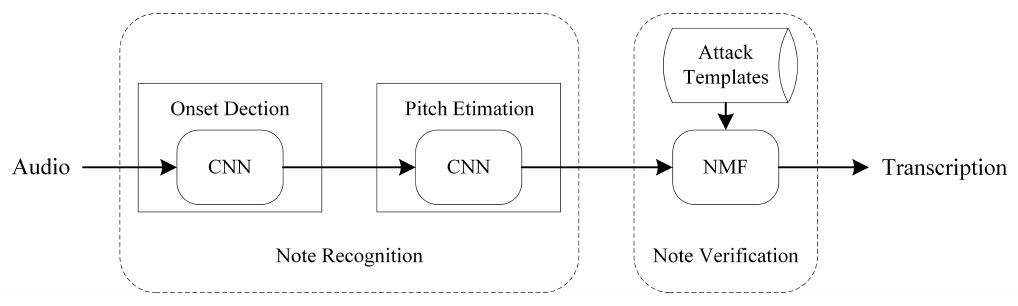
\includegraphics[width=12cm]{./statics/wang2017two_architecture.png}
    \caption{ساختار مدل استفاده شده در \cite{wang2017two}}
\end{figure}

در \cite{hawthorne2017onsets} این ایده مطرح شد که همه فرم‌‌های ورودی ارزشی برابر
ندارند. فرم‌هایی که در آن‌ها نتی شروع می‌شود باید با اهمیت بالاتری بررسی شوند.
دلیل اصلی این دعا شکلی است که صوت در ساز پیانو تولید می‌شود. زمانی که یک کلاویه
پیانو فشرده می‌شود، صدا شدت بسیار بالاتری نسبت به ادامه دارد. به این مرحله از
تولید صوت، مرحله حمله نیز می‌گویند. پیشنهاد داده شده این بود که ابتدا یک شبکه
فقط شروع نت‌ها را تشخیص دهد و سپس از این اطلاعات به دست آماده برای تشخیص فعال
بودن یا نبودن نت‌ در فرم‌ها بعدی استفاده شود. به تعبیری تنها در صورتی در فرم‌های
بعدی یک \gls{pitch} فعال در نظر گرفته می‌شود که در فرم‌های قبلی شبکه تشخیص داده
باشد که آن نت شروع شده است.

در این سیستم، در قدم اول با استفاده از مقیاس mel و \gls{STFT} یک نمایش
زمان-فرکانس از سیگنال ورودی به دست می‌یاد. این نمایش به دست‌آمده ۲۲۹ دسته‌بندی
فراکانس دارد. سپس این نمایش به دست آمده به \gls{cnn} داده می‌شود که ساختاری
مشابه مدل پیشنهادی در \cite{kelz2016potential} دارد. خروجی این شبکه به یک شبکه
\gls{blstm} داده می‌شود. هر جهت این شبکه دارای ۱۲۸ نرون است. در نهایت هر فرم به
یک شبکه \gls{fully connected} داده می‌شود که ۸۸ نرون خروجی دارد. این نرون‌ها از
تابع سیگموید به عنوان تابع فعال‌سازی استفاده می‌کنند. این خروجی شروع نت‌ها را
مشخص می‌کند. اگر مقدار هر خروجی در یک فرم بیشتر از حدآستانه باشد، نت متناظر در
این فرم فعال می‌شود.

از \gls{cnn} دیگر برای تشخیص نت‌های فعال استفاده می‌شود. این شبکه این ساختاری
معادل \gls{CNN} قبلی دارد. پس از دادن نمایش زمان-فرکانس به این شبکه، خروجی به یک
شبکه \gls{fully connected} با ۸۸ نرون خروجی و تابع فعال‌سازی سیگموید داده
می‌شود. در نهایت خروجی به دست آمده از این شبکه همراه با خروجی به دست آمده از بخش
تشخیص شروع نت، به یک شبکه \gls{blstm} داده می‌شود. در نهایت پس از اعمال یک شبکه
\gls{fully connected} دیگر بر روی خروجی، فعال بودن یا نبودن هر نت در هر فرم مشخص
می‌شود. در شکل زیر ساختار کلی شبکه نشان داده است.
\begin{figure}[ht]
    \centering
    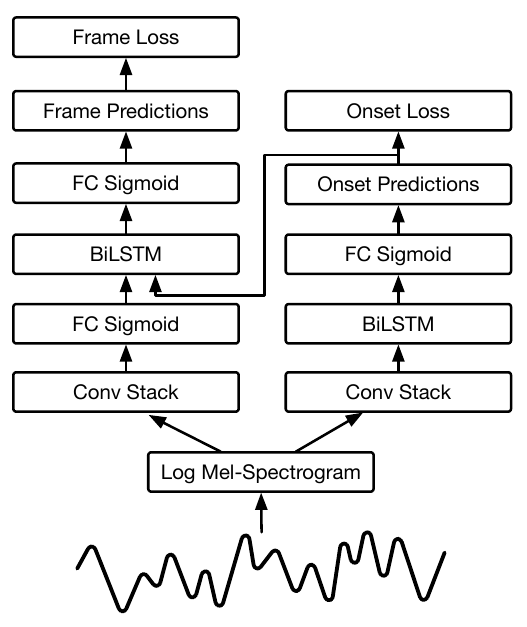
\includegraphics[height=8cm]{./statics/onset_onframe_architecture.png}
    \caption{ساختار شبکه استفاده شده در \cite{hawthorne2017onsets}}
\end{figure}

وقتی که شروع نتی تشخیص داده شود، نت فعال می‌مانند تا در فرم وجود نت تشخیص داده
نشود یا شروع جدید برای آن نت تشخیص داده شود.

برای آموزش شبکه از هر دو خروجی استفاده می‌شود. همچنین هر خروجی به کمک تابع خطا
\gls{cross entropy} استفاده می‌شود که در روابط زیر نشان داده است:
\begin{equation}
    L_{total} = L_{onset} + L_{frame}
\end{equation}
\begin{equation}
    L_{onset} = \sum_{p=1}^{88} \sum_{t=0}^{T} W(p, t) CE(I_{onset}(p, t), P_{onset}(p, t))
\end{equation}
\begin{equation}
    L_{frame} = \sum_{p=1}^{88} \sum_{t=0}^{T} W(p, t) CE(I_{frame}(p, t), P_{frame}(p, t))
\end{equation}
\begin{equation}
    W(p, t) =
    \begin{cases}
        c &\quad t = t_{onset}\\
        \frac{c}{t - t_{onset}} &\quad t_{onset} \leq t \leq t_{offset}\\
        1 &\quad \text{otherwise}
    \end{cases}
\end{equation}

$I_{onset}$ تابع مشخصه شروع شدن نت $p$ در فرم $t$ است. $I_{frame}$ تابع مشخصه
فعال بودن نت $p$ در زمان $t$ است. همچنین $P_{onset}$ و $P_{frame}$ به ترتیب
خروجی‌های شروع و فعال بودن نت‌ها شبکه است. همچنین $c$ یک مقدار ثابت است که برابر
۵/۰ است.

با توجه مصرف بالای حافظه شبکه‌های \gls{LSTM} بر روی دنباله‌های ورودی طولانی، هر
قطعه به صورت کامل امکان نمایش به مدل را ندارد. برای همین هر قطعه به برش‌هایی به
طول حداکثر ۲۰ ثانیه تقسیم شده است. برای برش تلاش شده است که در تنهایی جایی اعمال
شود که هیچ نت فعالی وجود ندارد. در نتیجه شبکه اطلاعات شروع نت‌ها را همچنین داشته
باشد. ولی در مرحله ارزیابی، هر قطعه به صورت کامل به مدل داده می‌شود.

در راستای طبیعی‌تر کردن خروجی سیستم، سیستم علاوه بر \gls{pitch}، شروع و پایان
نت‌ها، تلاش می‌کند که \gls{velocity} نت‌ها را نیز تشخیص دهد. \gls{velocity} هر
نت تاثیر بسیار بسازی در درک ما از موسیقی دارد و یک آوانویسی کاملا نیاز دارد تا
اطلاعات مرتبط با \gls{velocity} را نیز شامل شود. یکی از چالش‌های پیشروی پیش‌بینی
\gls{velocity} نت‌ها این است که این ویژگی یک مقدار کاملا نسبی هست. دو نوازنده
ممکن است یک قطعه را با قدرت کاملا متفاوت اجرا کنند، ولی همچنان \gls{velocity}
نت‌ها را کاملا رعایت کرده باشند. سیستم برای پیش‌بینی این مقدارها ابتدا
\gls{velocity} نسبت داده شده بر هر نت در فایل \gls{MIDI} را بر حداکثر مقدار ظاهر
شده در فایل تقسیم می‌کند. در نتیجه به هر نت مقدار ما بین صفر و یک نسبت داده می
شود. در مرحله بعد از شبکه‌ای با ساختاری بسیار نزدیک به ساختار استفاده برای
پیش‌بینی شروع نت‌ها استفاده می‌شود تا مقدار \gls{velocity} هر نت را در زمان شروع
نت، تشخیص داده شود. این شبکه عمل \gls{regression} را انجام می‌دهد و با سایر
شبکه‌های استفاده در سیستم ارتباطی ندارد.

برای آموزش از تابع خطای زیر استفاده می شود:
\begin{equation}
    L_{vel} = \sum_{p=1}^{88} \sum_{t=0}^{T} I_{onset}(p, t) (v_{label}^{p,t} - v_{predicted}^{p,t})^{2}
\end{equation}
که $v_{label}^{p, t}$ مقدار واقعی \gls{velocity} نت است که مقداری بین صفر و یک
دارد. $v_{predicted}^{p,t}$ مقدار پیش‌بینی شده شبکه است. با ضرب این مقدارها در
$I_{onset}(p, t)$ می‌توان مطمئن شد که شبکه فقط از شروع نت‌ها برای پیش‌بینی
\gls{velocity} هر نت استفاده کند. در نتیجه می‌توان انتظار دقت بالاتری از این پیش‌بینی داشت.

پس از آموزش، برای تبدیل این مقدارهای خروجی شبکه به مقدار \gls{velocity} استفاده
شده در آوانویسی خروجی، از رابطه زیر استفاده می‌شود:
\begin{equation}
    v_{midi} = 80 v_{predicted} + 10
\end{equation}
هر چند که هیچ دلیل علمی برای استفاده از ۸۰ و ۱۰ به عنوان مقدارهای این تبدیل خطی
وجود ندارد، ولی از آزمایش‌ها این مقدارها معمولا باعث تولید آوانویسی خوش‌آیند
شده‌اند.

با توجه به مشکلات مربوط به \gls{dataset} که در \cite{hawthorne2017onsets} مطرح
شده بود، \cite{hawthorne2018enabling} در قدم اول تلاش کرد با معرفی \gls{dataset}
جدید دقت مدل را افزایش دهد. این \gls{dataset} جدید شامل بیش از یک هفته موسیقی
است که طی نه سال جمع آوری شده است و از خطاهای موجود در \glspl{dataset} پیشین رنج
نمی‌برد.

همچنین تلاش شده که با ایجاد تغییراتی در مدل پیشنهاد شده توسط
\cite{hawthorne2017onsets} دقت افزایش پیدا کند. مهم‌ترین این تغییرات افزودن بخش
جدید به شبکه بود که وظیفه تشخیص پایان نت‌ها را دارد. این بخش جدید ساختاری کاملا
مشابه بخش تشخیص شروع نت‌ها دارد و خروجی آن همچنین به بخش تشخیص فعال بودن نت‌ها
داده می‌شود. در سازهایی همچون پیانو که نت‌ها حتی پس از رها کردن کلاویه همچنان
فعال می‌مانند صوتی تولید می‌کنند، می‌تواند بسیار به عملکرد نهایی مدل کمک کند.
این بخش از شبکه می‌توان افت در صوت ورودی را تشخیص دهد و متوجه شود که کلاویه رها
شده است. همچنین در طی آوانویسی اگر این خروجی تشخیص دهد نتی پایان یافته است، نت
پایان‌یافته فرض می‌شود حتی اگر خروجی اصلی فعال بودن نت را همچنان تشخیص دهد.

از جمله تغییرات دیگر می‌توان به افزایش اندازه شبکه‌های \gls{CNN} و \gls{BLSTM}
استفاده شده اشاره کرد که با توجه به افزایش حجم داده‌ای که مدل برای آموزش استفاده
می‌کند، می‌توان تاثیر خوبی بر افزایش دقت داشته باشد. همچنین در این مدل در هنگام
آموزش به گرادیان‌های بخش تشخیص فعال بودن نت‌ها اجازه نفوذ به سایر بخش‌ها داده
نمی‌شود و بخش‌های دیگر فقط با استفاده از تابع خطای متناظر خودشان آموزش داده
می‌شوند.

همچنین پیشنهاد داده شد تا از روش‌های تشدید داده استفاده شود تا مقاوت مدل افزایش
یابد و قابلیت تعمیم آن افزایش دهد. برای این منظور از نرم‌افزار SoX استفاده شد و
هر نمونه آموزشی توسط پارامترهایی که مقدار آن‌ها به صورت تصادفی انتخاب می‌شود
مقداری تغییر می‌کند. نتیجه بر خلاف انتظار باعث کاهش در دقت نهایی شد در نتیجه در
مدل نهایی از تشدید داده استفاده نمی‌شود.

در \cite{kim2019adversarial} این ایراد به مدل‌های معرفی شده گرفته شد که تابع خطا
برای هر فرم و نت به صورت جدا محاسبه می‌شود در نتیجه رابطه بین نت‌ها و فرم‌های
مختلف در آموزش در نظر گرفته نمی‌شود. برای حل این مشکل پیشنهاد داده شد تا از
\gls{cgan} برای طراحی یک سیستم \gls{atm} استفاده شود. با استفاده از این ساختار،
مدل \gls{discriminative} می‌تواند روابط بین نت‌های مختلف را نیز فرابگیرد و برای
آوانویسی مدل از این روابط استفاده کند.

بخش \gls{generative} ساختاری کاملا مشابه به مدل معرفی شده در
\cite{hawthorne2018enabling} دارد. این مدل سیگنال صوتی را می‌گیرد و خروجی
آوانویسی با ساختاری شبیه به \gls{pianoroll} ارائه می‌دهد. در شکل زیر نمایی از
بخش \gls{generative} نشان داده شده است.
\begin{figure}[ht]
    \centering
    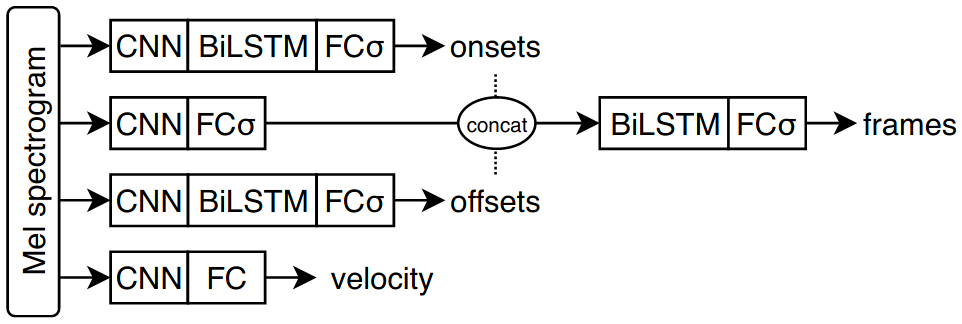
\includegraphics[width=12cm]{./statics/kim2019adversarial_generative_architecture.png}
    \caption{ساختار مدل \gls{generative} استفاده شد در \cite{kim2019adversarial}}
\end{figure}

بخش \gls{discriminative} بر خلاف مدل‌های مشابه، آوانویسی ساخته شده و آوانویسی
واقعی‌ای را از ورودی می‌گیرد. گرفتن آوانویسی بجای سیگنال ورودی باعث می‌شود که
مدل تنها کافی باشد که یادبگیرد آیا تو آوانویسی معادل هستند یا نه و نیازی به
یادگیری انجام آوانویسی نداشته باشد. این بخش از سیستم کاملا بر پایه \gls{cnn}
ساخته شده است و شامل پنج لایه می‌شود. در نهایت خروجی مدل میانگین تمام خروجی‌های
لایه آخر است. در شکل زیر ارتباط این بخش با بخش \gls{generative} نشان داده شده
است.
\begin{figure}[ht]
    \centering
    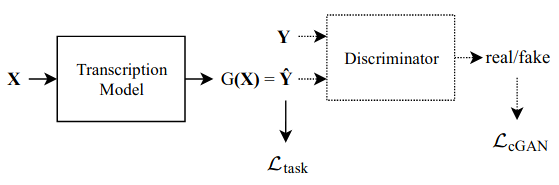
\includegraphics[width=12cm]{./statics/kim2019adversarial_architecture.png}
    \caption{شکل ارتباط بخش‌های \gls{generative} و \gls{discriminative} در \cite{kim2019adversarial}}
\end{figure}

\cite{roman2018end} بجای استفاده از \gls{pianoroll} به عنوان یک نمایش میانی برای
آوانویسی، تلاش می‌کند که مستقیم \gls{sheet music} را تولید کند. برای تولید
\gls{sheet music} از روی \gls{pianoroll} مسائل مختلفی مانند تشخیص ریتم، تشخیص
کلید و تشخیص کشش‌ها بر اساس ریتم نیاز است که حل شود. تولید مستقیم \gls{sheet
music} نیاز به حل این مسائل در سیستم‌های مجزا را از بین می‌برد. همچنین نیاز به
\gls{dataset} که برچسب‌ها کاملا از نظر زمانی منطبق بر صوت ضبط شده باشند را نیز
منتفی می‌کند. در نتیجه می‌توان از داده‌های بسیار بیشتری برای آموزش سیستم استفاده
کرد. یکی دیگر از مشکلات تولید \gls{pianoroll} به عوان واسط سخت‌تر شدن تشخیص کشش
نت‌ها بر روی سازهای زهی مانند گیتار است. سیستمی که مستقیم \gls{sheet music} را
تولید می‌کند می‌تواند این تشخیص را بهره بردن از اطلاعات موسیقی مانند تعداد نت‌ها
در هر میزان انجام دهد.

برای رسیدن به این هدف ابتدا فرض شده که تمام ورودی‌ها \gls{monophonic} هستند. هر
چند مسئله \gls{atm} برای قطعات \gls{monophonic} مدت زیادی هست که حل شده فرض
می‌شود ولی تولید مستقیم \gls{sheet music} بجای استفاده از یک نمایش واسط سختی
مسئله را چندین برابر می‌کند. از این جهت حتی با این وجود این فرض، مسئله همچنان
بسیار چالش برانگیز باقی می‌ماند.

برای آموزش شبکه، ابتدا از \gls{dataset} RISM استفاده می‌شود که شامل تعداد زیادی
\gls{sheet music} از شروع قطعات واقعی است. به کمک نرم‌افزارهای شبیه‌ساز از روی
\gls{sheet music} موجود، خروجی صوتی اجرای آن‌ها تولید می‌شود. از سیگنال‌های صوتی
به دست آمده استفاده می‌شود تا یک نمایش زمان-فرکانس به کمک \gls{STFT} به دست آید
که ورودی شبکه است. سپس شبکه تلاش می‌کند از روی این نمایش‌های به دست آمده
\gls{sheet music} استفاده شده برای تولید قطعه را حدس بزند. شکل زیر نمای کلی این
فرآیند را نشان می‌دهد.
\begin{figure}[ht]
    \centering
    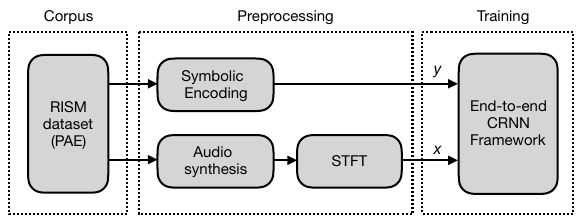
\includegraphics[width=12cm]{./statics/roman2018end_architecture.png}
    \caption{نمایی از سیستم معرفی شده در \cite{roman2018end}}
\end{figure}

شبکه معرفی شامل چند لایه \gls{CNN} است که خروجی آن‌ها به چند لایه \gls{BGRU}
داده می‌شود. به \gls{cnn} نمایش زمان-فرکانس محاسبه شده داده می شود. این لایه‌ها
تلاش می‌کنند اطلاعات مهم را از نمایش ورودی استخراج کنند. سپس با کمک گیری از
\gls{BGRU} این ویژگی‌های استخراج شده به دنبالی از نمادها تبدیل می‌شود که با همان
ترتیب \gls{sheet music} را شکل می‌دهند. همچنین برای تابع خطا از \gls{CTC}
استفاده می‌شود که نیاز به منطبق بودن خروجی ها با فرم‌های ورودی را از بین می‌برد.

با بررسی‌های انجام شده بر روی آوانویسی‌های انجام مشخص شد که مشکل اصلی مدل در
تشخیص ریتم و کلید هر ورودی است. با توجه به این که ورودی‌ها به صورت عمده از ضرب
۴/۴ تشکیل شده‌اند، این رفتار کاملا قابل انتظار هست. برای تشخیص کلید هر قطعه و
ریتم استفاده شده حتی موسیقدانان خبره نیز به اطلاعات بسیار بیشتری نیاز دارند. در
صورتی که کلید و ریتم هر قطعه دستی اصلاح شود، مدل خروجی قابل قبولی تولید می‌کند و
می‌تواند کشش و \gls{pitch} هر نت را به خوبی تشخیص داده و خروجی \gls{sheet music}
تا حد زیادی نزدیک با واقعیت است. در شکل زیر نمونه‌ای خروجی سیستم هست که این
موضوع را به خوبی نشان می‌دهد.
\begin{figure}[ht]
    \centering
    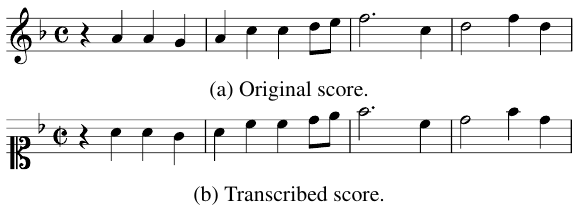
\includegraphics[width=12cm]{./statics/roman2018end_output.png}
    \caption{نمونه‌ای از آوانویسی انجام شده توسط \cite{roman2018end}}
\end{figure}

در نهایت هر چند دقت نهایی این سیستم هنوز قابل مقایسه با سایر سیستم‌های پیش‌بینی
شده نیست، ولی نتایج به دست آمده به خوبی نشان می‌دهند که تولید مستقیم \gls{sheet
music} به کمک \gls{dl} کاملا شدنی است و می‌توان به عنوان جایگزینی برای روش‌های
موجود به بررسی بیشتر این خانواده از روش‌ها پرداخت.

\section{مقایسه روش‌های براساس تحزیه نامنفی ماتریس و شبکه عصبی}
با توجه به محبوبیت \gls{nmf} و \gls{nn} برای حل مسئله \gls{atm} در ادامه به
بررسی تفاوت‌های این دو روش می‌پردازیم.

\gls{NMF} یک مدل خطی هست در حالی که \gls{NN} مدلی کاملا غیرخطی محسوب می‌شود.
اولین سوالی که مطرح می‌شود این هست که آیا این خطی بودن محدودیتی ایجاد خواهد کرد
یا نه. فرض کنید که به ازای هر \gls{pitch} دو قالب اسپکترال داریم. برای نمایش
\gls{spec} یک نت، دو قالب موجود را به صورت خطی با هم ترکیب می‌کنیم. ولی مجموعه
\gls{spec} متناظر با هر نت بسیار پیچیده‌تر هست و معمولا یک ترکیب خطی از آن‌ها
معادل یک ضبط واقعی نخواهد بود. می‌توانیم تعداد قالب‌های هر \gls{pitch} را افزایش
دهیم و مجددا تعداد نمایش‌ها نامعتر تولید شده بسیار بیشتر از نمایش‌ها معتبر خواهد
بود. از طرف دیگر \gls{nn} در سال‌های اخیر توانایی خوبی در نمایش این چنین
داده‌هایی را به صورت مقاوم و نسبت بهینه نشان داده‌اند \cite{goodfellow2016deep}.

یک مزیت دیگر مدل‌های برپایه \gls{NN} قابل آن‌ها برای آموزش به صورت \gls{e2e}
است. به این صورت که خروجی مدل می‌تواند مستقیم نت‌های تشخیص داده شده باشد و نیازی
به یک مرحله پس‌پردازش اضافه که در مدل‌های بر اساس \gls{NMF} لازم هست، نباشد.

با این وجود روش‌های مبتنی بر \gls{NMF} دو مزیت دارند که باعث می‌شود همچنان از
آن‌ها استفاده شود و نتایج قابل قبولی هم به دست آورند. مشکل اولی که در مقابل
\gls{nn} قرار دارد، کمبود دیتای مناسب هست. حتی بزرگ‌ترین \glspl{dataset} موجود
نیز در حد چند ساعت اطلاعات دارند. همچنین این دادگان از مشکل بایاس شدید رنج
می‌برند. شرایط ضبط هم معمولا تنوع لازم را ندارند و معمولا در چند محیط خاص و مدل
خاص ضبط انجام شده است. این محدودیت‌ها باعث می‌شود که همیشه خطر \gls{overfit}
وجود داشته باشد. همچنین برای بسیاری از سازها در لحظه هیچ \gls{dataset} وجود
ندارد.

مشکل دیگری که روش‌های مبتنی بر \gls{nn} از آن رنج می‌برند قابلیت تعمیم به شرایط
آکوستیکی جدید هست. معمولا مدل‌های برپایه \gls{nmf} موجود می‌تواند تنها با
استفاده از چند ثانیه از داده نواختن یک ساز جدید نتایج قابل قبولی بر ساز جدید
نمایش دهند. در لحظه هیچ شاهدی مبنی بر تونایی مشابه در روش‌های بر پایه \gls{NN}
ارائه نشده است. این مهم باعث می‌شود که روش‌های مبتنی بر \gls{NMF} همچنان به صورت
گسترده مطالعه شوند و مورد استفاده قرار گیرند.

\section{جمع‌بندی}
در این فصل بر مسئله آوانویسی گفتار نگاه دقیق‌تری انداخته شد و با مهم‌ترین
تلاش‌های گذشته در جهت حل این مسئله آشنا شدیم. سطح‌های حل مسئله معرفی شدن و
دسته‌بندی کلی بر روش‌های حله این مسئله ارائه شد. سپس مروری کلی بر روش‌های
\gls{nmf} انجام شد. سپس مهم‌ترین مدل‌های براساس \gls{nn} بررسی شدند. در نهایت
مقایسه‌ای مابین روش‌های مبتنی بر \gls{nmf} و روش‌های مبتنی بر \gls{nn} انجام شد
و با معایب و مزایای هر کدام آشنا شدیم.